% Welfare of per-driver fill rates (analyze/welfare_analysis.py).
\begin{figure}[H]
    \centering
    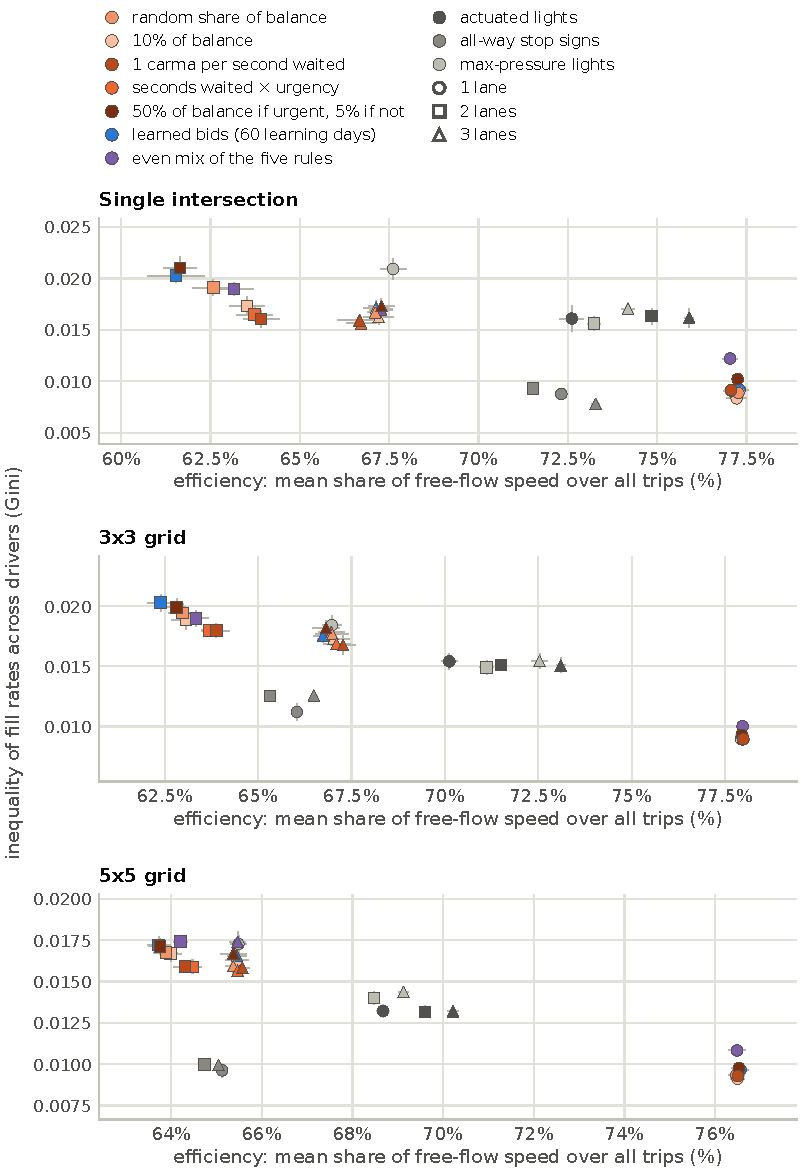
\includegraphics[width=\linewidth]{welfare_efficiency_equity.pdf}
    \caption{Efficiency against equity of per-driver fill rates (eq.~\eqref{eq:welfare}): each
    point is a strategy at one lane count; right is more efficient (trips run at a larger share of
    free-flow speed), low is more equal (smaller Gini of drivers' average share). A driver's need
    is their number of trips. Reference setting, the same 7-day evaluation week for every
    strategy (fixed rules after 7 warm-up days, learned bids after 60 learning days); means of
    10 seeds, whiskers 95\% intervals; each panel has its own scales.}
    \label{fig:welfare}
\end{figure}
